\chapter{Architecture \& Implementation}
\label{chap:implementation}

We will look into the details of each component of the system and how they are implemented.
Then we will discuss the higher level architecture of the system and how the components interact with each other.

\section{Proof of Retrievability}

Proof of Retrievability\cite{porfirst} (PoR) is a protocol that allows a client to verify that a server is storing a file correctly.
The client can do this without downloading the entire file.
While this protocol is meant to be used in a client-server setting, we can use it in a peer-to-peer setting.
The clients are the Verifiers and the servers are the Keepers.

Some PoR protocols allow file updates or even partial file updates, however we do not use these features.
The update procedure is often expensive and complex.
Instead, we can use Kademlia to store the file and update it if necessary.
The only part we are changing from Kademlia is the way the file is stored.
Instead of storing the file directly, we perform a preprocessing step, providing us with the metadata needed for the PoR protocol.
Then we store the metadata in the ledger/catalog and the file in the DHT.
Later we can use the metadata to verify the file in the DHT.

This is not secure once again since the Keeper and Verifier nodes are conjoined.
PoR protocols are designed to be secure against malicious servers, but not malicious clients.
In our case, a malicious Keeper can use their Verifier to retrieve the metadata from the ledger and break the PoR protocol.
However, modern PoR protocols propose a public auditability feature that allows anyone to verify the file.
This would make the protocol secure against malicious Keepers.
We do not implement this feature in our system, because of the complexity it adds to the protocol.
We leave it to future work.

The PoR protocol we are using is based on the one described in Dynamic proofs of retrievability with low server storage\cite{poralgebra}.
The full protocol is described in the paper, so we will only describe some important parts.
The protocol treats the input file as a matrix of bytes with $n$ rows and $m$ columns.
The parameter $n$ is related to the security of the protocol as well as the size of the metadata that the client needs to store.
The parameter $m$ is related to the size of the messages that need to be exchanged during the verification/audit step.
To balance the security and the efficiency of the protocol, we need to choose the parameters $n$ and $m$ carefully.
In practice, it makes sense to choose them such that $n \approx m$.

The procedure of the protocol is as follows:

\begin{center}
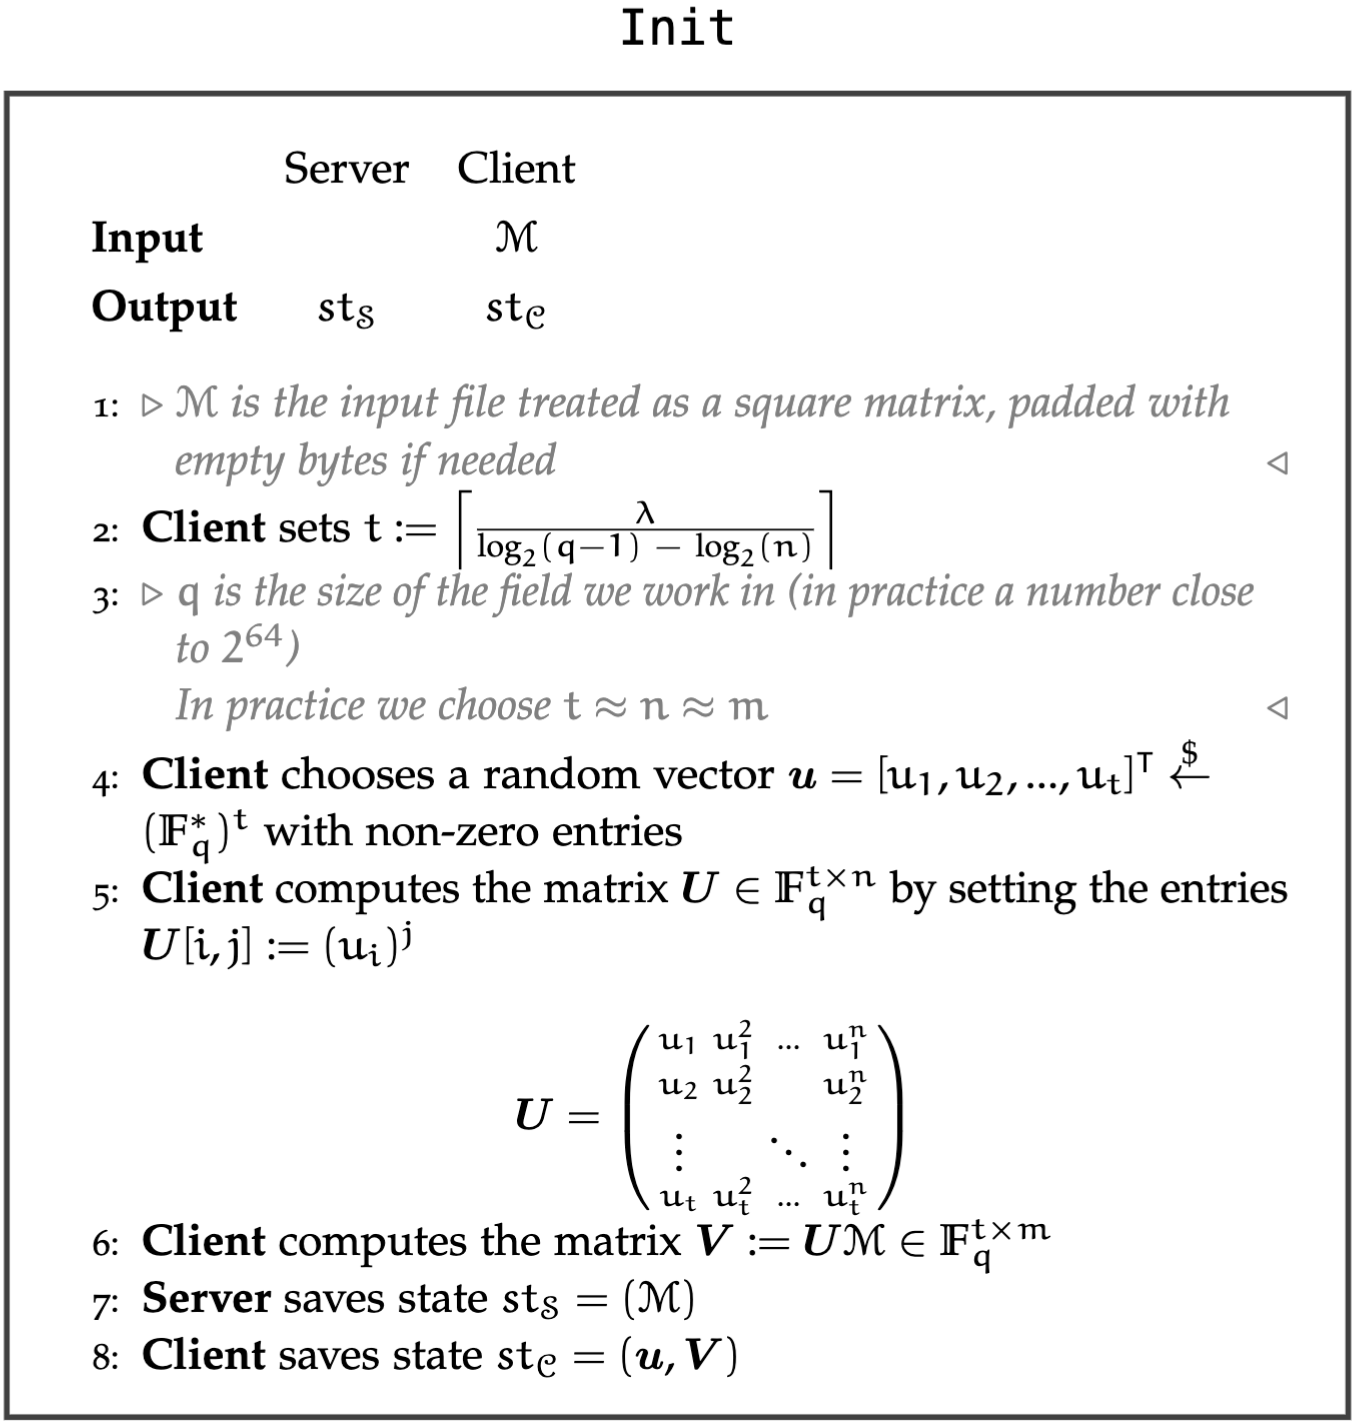
\includegraphics[width=\textwidth,height=\textheight,keepaspectratio]{init}
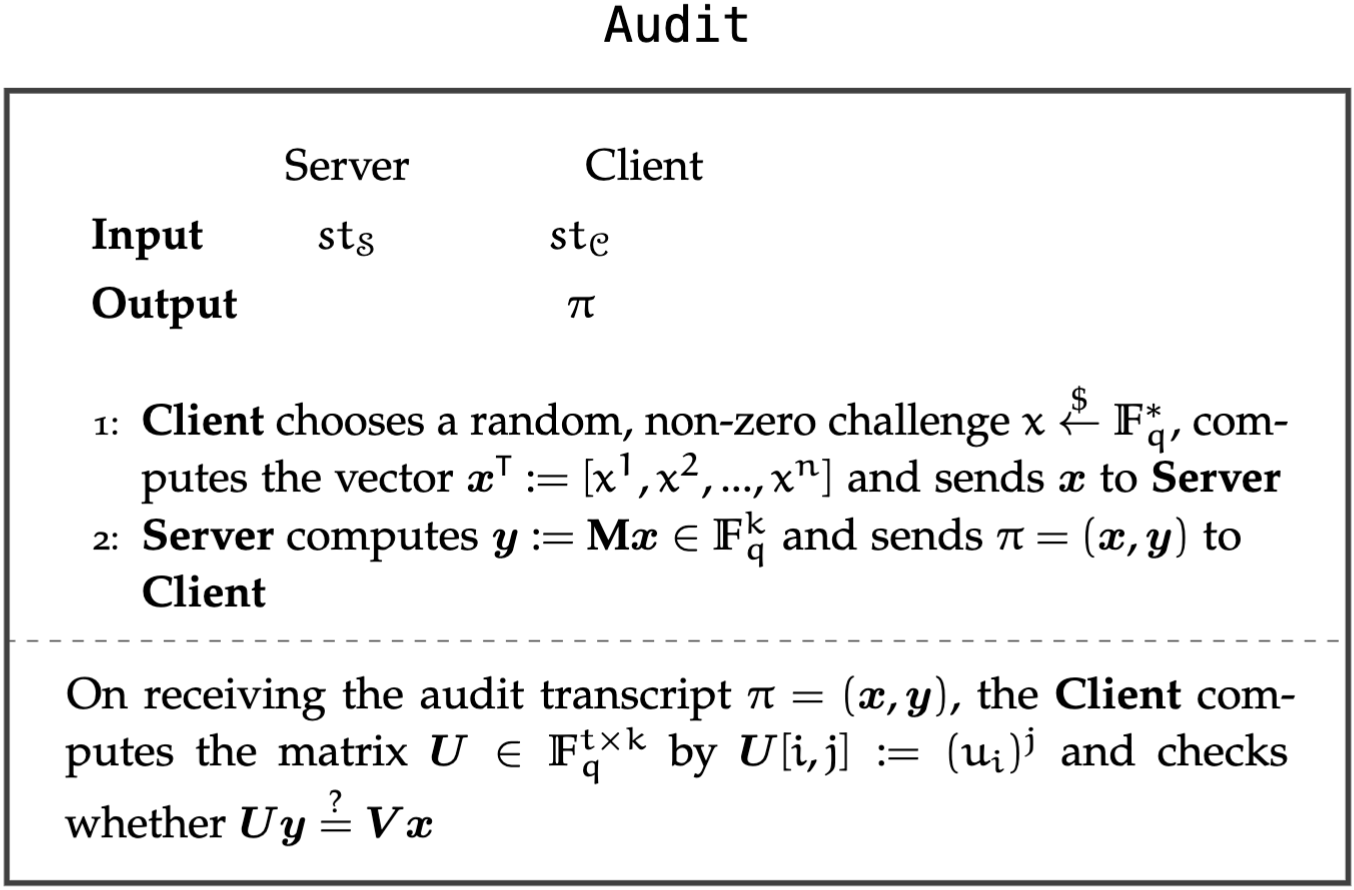
\includegraphics[width=\textwidth,height=\textheight,keepaspectratio]{audit}
\end{center}

We have implemented the PoR protocol, closely following the paper and the implementation by the authors.
This choice was made, so we can compare our results with theirs and ensure that our implementation is correct.
It is important to note that the original implementation uses the Mersene Twister random number generator.
This is not a cryptographically secure PRNG, so we have replaced it with the ChaCha20 PRNG\cite{chacha}.


Other minor differences are:
\begin{enumerate}
    \item Unlike the original implementation, we do not parallelize the multiplication of the matrices,
        which makes our implementation slower.
        This is something we leave for future work.
    \item We have to use more modulo operations to ensure the calculations do not overflow.
        The original algorithm sometimes allows overflows, but these are not allowed in Rust.
        If an overflow happens in Rust, the program will crash.
    \item We are hard-coding the values that the original hard-coded as well, which are needed to argue about the security.
    \item Instead of relying on custom read functions, we pad the file with empty (zero) bytes to enable proper alignment.
        This is done only when calculations are performed and never affects the file.
\end{enumerate}

\section{Local Storage}

The default Kademlia implementation of the storage is an in-memory storage.
This means that the data does not persist and is lost when the program (peer) is closed.
This is not suitable for our use case, because we want to store the files persistently, even between peer restarts.
To achieve this, we have implemented a local storage module, which uses the file system to store the files.
The module is implemented to adhere to the Kademlia storage interface, so it can be used as a drop-in replacement for the in-memory storage.
Underneath, it uses the \texttt{object\_store} crate, which provides an S3-like interface for storing objects.
This allows us to easily switch between local storage and cloud storage.

We had to implement a wrapper around the \texttt{object\_store} crate for two reasons.
First, we wanted to be able to store and retrieve files that adhere to a custom structure.
Second, while Kademlia is asynchronous, it requires a synchronous storage interface.
However, the \texttt{object\_store} crate is asynchronous, so we had to wrap it in a synchronous interface.
This posed difficulties because the \texttt{object\_store} was also shared between threads.
The solution was to use a reference-counted pointer wrapped in a mutex to the \texttt{object\_store}.
This allows us to clone the pointer and lock the mutex when we need to use the \texttt{object\_store}.
The mutex is locked throughout the whole operation of reading/writing a file.
This is a downside of the implementation because it means that only one thread can read/write a file at a time.
However, in practice, multithreaded access to local storage is slow and does not provide any benefits.

We are saving the files named by their unique identifiers.
This allows us to quickly check if a file is stored at a peer by checking if the file exists, without keeping a separate index.

Kademlia has a concept of a Record and not a file.
A Record is a key, a value, a publisher, and an expiration time.
Since we are working in Rust, we cannot dump the memory of a struct to a file and read it back.
Instead, we have to serialize the Record to a string or a byte array and then deserialize it back.
We have opted to use YAML as the serialization format because it is human-readable and easy to debug.
The serialization and deserialization are done using the \texttt{serde} crate, which provides a framework for serializing and deserializing Rust data structures efficiently and generically.
The one downside is that in Rust, you cannot implement a trait (interface) for a type that is not defined in your crate/project.
This means that we cannot implement the \texttt{serde} traits for the \texttt{Record} struct, because it comes from the \texttt{kademlia} crate.
To resolve this, we have created a wrapper struct around the \texttt{Record} struct, which implements the \texttt{serde} traits.
Serializing the key and publisher is not straightforward, but both are byte arrays, which can be converted to strings, and strings are serializable.
The problematic part is the expiration time, which is an \texttt{Instant}.
This is a struct that represents a point in time, but it is not serializable, because it is not convertible to a timestamp.
It is meant to be used as an opaque type, which is only used for comparisons.
To resolve this, we are sacrificing part of the precision of the expiration time, by converting it to a timestamp manually.
While this is not an ideal solution, in practice it will have only a few milliseconds of error, which is acceptable.
The value is a byte array, which we serialize by encoding to base64.
While this is not the most efficient way to serialize the value, it is the easiest to implement.
In a future version, we would separate the value from the rest of the record and store it as a binary file.

\section{Cryptographic puzzle}

The cryptographic puzzle is a proof-of-work algorithm that is used to prevent Sybil attacks.
Before a peer can join the network, they need to generate a peer ID.
During this step, they are required to solve a cryptographic puzzle.
Our implementation is in two steps.
First, we generate a random peer ID using an ED255519 elliptic curve algorithm.
Then we hash the peer ID using SHA-3 and expect the hash to start with a certain number of zeros.
The number of zeros is a parameter of the puzzle and is related to the security of the puzzle.
If the hash does not start with the required number of zeros, we generate a new peer ID and try again.

This is easily verifiable by other peers because they can hash the peer ID and check if the hash starts with the required number of zeros.
This is also a computationally expensive task because the only way to find a peer ID that satisfies the puzzle is to generate random peer IDs and hash them until we find one that satisfies the puzzle.
We will discuss the number of zeros in the puzzle in the evaluation section.

\section{Decentralized Verifier}

The decentralization of the Verifier is by far the most impactful change we have made to the system.
In Version 1, the Verifier was a centralized entity that was responsible for verifying the files.
This was a single point of failure because if the Verifier were down, the system would not work.
Also, it did not make sense for a decentralized system to have a centralized entity (authority).
In Version 2, we are moving towards a decentralized Verifier.
The Verifier is now a logical part of every node in the system.

To achieve this, we merged the verifier module with the keeper module.
In the previous version, the Verifier contacted the Keeper nodes via GRPC over TCP.
Now the verifier can access the Kademlia interface and interact with peers via the Kademlia protocol.
This means we had to rework the Contracts for storing a file, which kept track of the Keeper's IP address,
but now only keep track of the Keeper's peer ID in the network.

In the implementation of Kademlia we are using PUT queries to store the file at the peer that received the query.
To store the file with other peers and achieve replication, we need to send PUT queries to other peers, which are called PUT\_TO queries.
There is a slight issue with this query because it reuses the response of the PUT query, which does not contain the peer IDs of the peer where the file is stored.
To circumvent this issue, we are making use of the GET\_CLOSEST\_PEERS query, which returns the peer IDs of the $k$ closest peers to a given key.
We then issue PUT\_TO queries to the $k$ closest peers and note down which peers have stored the file.
Now we have a list of peers that have stored the file, with which we can create the Contracts and, later on, use them to verify the file.
The final thing that allows us to use this approach is the fact that the GET query returns the peer ID that answers the query.
This allows us to issue verification requests using the GET query to the peers that have stored the file, and get information about which peers answer the query.
